\hypertarget{libphonefirewall_8h}{
\section{libphonefirewall.h File Reference}
\label{libphonefirewall_8h}\index{libphonefirewall.h@{libphonefirewall.h}}
}
API of the phone firewall. 



This graph shows which files directly or indirectly include this file:\nopagebreak
\begin{figure}[H]
\begin{center}
\leavevmode
\includegraphics[width=226pt]{libphonefirewall_8h__dep__incl}
\end{center}
\end{figure}
\subsection*{Data Structures}
\begin{CompactItemize}
\item 
struct \hyperlink{structEntry}{Entry}
\end{CompactItemize}
\subsection*{Defines}
\begin{CompactItemize}
\item 
\#define \hyperlink{libphonefirewall_8h_6265f3115ead4b41b74ad4b8fe53a801}{PRIO\_\-ALL}~-999
\item 
\#define \hyperlink{libphonefirewall_8h_ee925031172607ff8d5cf8b68374bd7f}{DB\_\-FILE}~\char`\"{}db/phone-firewall.db\char`\"{}
\item 
\#define \hyperlink{libphonefirewall_8h_8d8e3d24a53ab9fb36efc6e592076751}{STMT\_\-SIZE}~1024
\item 
\#define \hyperlink{libphonefirewall_8h_f0f2173e3b202ddf5756531b4471dcb2}{MAX\_\-LINE\_\-LENGTH}~512
\item 
\#define \hyperlink{libphonefirewall_8h_bfd305db409c094deb83b4714fb4fa09}{TB\_\-COUNTRYCODE}~\char`\"{}countrycode\char`\"{}
\item 
\#define \hyperlink{libphonefirewall_8h_c1694ee0c53e113107b2c0de64fc29a0}{TB\_\-AREACODE}~\char`\"{}areacode\char`\"{}
\item 
\#define \hyperlink{libphonefirewall_8h_01eced94590c7d08bd01ad7162bb47ad}{TB\_\-NUMBER}~\char`\"{}number\char`\"{}
\item 
\#define \hyperlink{libphonefirewall_8h_4f0324ecc491c659c1d250247ed4bb11}{TB\_\-NAME}~\char`\"{}name\char`\"{}
\item 
\#define \hyperlink{libphonefirewall_8h_769f1e2c007617c185b5a3c09229ee67}{TB\_\-REASON}~\char`\"{}reason\char`\"{}
\item 
\#define \hyperlink{libphonefirewall_8h_22e4a39534c1dcde6556befda55b4607}{TB\_\-PRIORITY}~\char`\"{}priority\char`\"{}
\end{CompactItemize}
\subsection*{Functions}
\begin{CompactItemize}
\item 
int \hyperlink{libphonefirewall_8h_36847ed3459e2a89038772ece42a017d}{add\_\-blacklist\_\-entry} (int country\_\-code, int area\_\-code, unsigned long long number, char $\ast$name, char $\ast$reason, int priority)
\item 
int \hyperlink{libphonefirewall_8h_4eee00c845ad4a60eaccef8c41151ea4}{rm\_\-blacklist\_\-entry} (int country\_\-code, int area\_\-code, unsigned long long number)
\item 
int \hyperlink{libphonefirewall_8h_f28c4b8fd3fdfe5e70df391cf40ca9f2}{check\_\-blacklist\_\-entry} (int country\_\-code, int area\_\-code, unsigned long long number, int priority)
\item 
int \hyperlink{libphonefirewall_8h_eec16cb88eb546b1a2490e6716d75f8b}{add\_\-whitelist\_\-entry} (int country\_\-code, int area\_\-code, unsigned long long number, char $\ast$name, char $\ast$reason, int priority)
\item 
struct \hyperlink{structentry}{entry} $\ast$ \hyperlink{libphonefirewall_8h_04b29323de592cc442250d7c952213de}{get\_\-blacklist\_\-entry\_\-by\_\-name} (char $\ast$name)
\item 
struct \hyperlink{structentry}{entry} $\ast$ \hyperlink{libphonefirewall_8h_80b7f603605d9ea57e83847bed7840f3}{get\_\-blacklist\_\-entry\_\-by\_\-number} (int country\_\-code, int area\_\-code, unsigned long long number)
\item 
int \hyperlink{libphonefirewall_8h_307d220ee8e63926af279460532787ff}{rm\_\-whitelist\_\-entry} (int country\_\-code, int area\_\-code, unsigned long long number)
\item 
int \hyperlink{libphonefirewall_8h_f144fe0aa2eb227fe646da21048388a5}{check\_\-whitelist\_\-entry} (int country\_\-code, int area\_\-code, unsigned long long number, int priority)
\item 
struct \hyperlink{structentry}{entry} $\ast$ \hyperlink{libphonefirewall_8h_f7f20dcd932db52fce6beac057995533}{get\_\-whitelist\_\-entry\_\-by\_\-name} (char $\ast$name)
\item 
struct \hyperlink{structentry}{entry} $\ast$ \hyperlink{libphonefirewall_8h_9569cf612525d13ec3443a5df88afe78}{get\_\-whitelist\_\-entry\_\-by\_\-number} (int country\_\-code, int area\_\-code, unsigned long long number)
\end{CompactItemize}
\subsection*{Variables}
\begin{CompactItemize}
\item 
struct \hyperlink{structEntry}{Entry} \hyperlink{libphonefirewall_8h_794ea73ef2f5143bbbb66ebd4c113340}{entry}
\end{CompactItemize}


\subsection{Detailed Description}
API of the phone firewall. 

\begin{Desc}
\item[Author:]Alex Oberhauser\end{Desc}
The header file of the Phone Firewall. Blocks or accepts incoming phone calls, so it's possible to prevent disturbing phone calls. Provides a API which can used by other application to build nice programs. 

Definition in file \hyperlink{libphonefirewall_8h-source}{libphonefirewall.h}.

\subsection{Define Documentation}
\hypertarget{libphonefirewall_8h_ee925031172607ff8d5cf8b68374bd7f}{
\index{libphonefirewall.h@{libphonefirewall.h}!DB\_\-FILE@{DB\_\-FILE}}
\index{DB\_\-FILE@{DB\_\-FILE}!libphonefirewall.h@{libphonefirewall.h}}
\subsubsection{\setlength{\rightskip}{0pt plus 5cm}\#define DB\_\-FILE~\char`\"{}db/phone-firewall.db\char`\"{}}}
\label{libphonefirewall_8h_ee925031172607ff8d5cf8b68374bd7f}




Definition at line 33 of file libphonefirewall.h.

Referenced by add\_\-blacklist\_\-entry(), add\_\-whitelist\_\-entry(), check\_\-blacklist\_\-entry(), check\_\-whitelist\_\-entry(), rm\_\-blacklist\_\-entry(), and rm\_\-whitelist\_\-entry().\hypertarget{libphonefirewall_8h_f0f2173e3b202ddf5756531b4471dcb2}{
\index{libphonefirewall.h@{libphonefirewall.h}!MAX\_\-LINE\_\-LENGTH@{MAX\_\-LINE\_\-LENGTH}}
\index{MAX\_\-LINE\_\-LENGTH@{MAX\_\-LINE\_\-LENGTH}!libphonefirewall.h@{libphonefirewall.h}}
\subsubsection{\setlength{\rightskip}{0pt plus 5cm}\#define MAX\_\-LINE\_\-LENGTH~512}}
\label{libphonefirewall_8h_f0f2173e3b202ddf5756531b4471dcb2}




Definition at line 35 of file libphonefirewall.h.\hypertarget{libphonefirewall_8h_6265f3115ead4b41b74ad4b8fe53a801}{
\index{libphonefirewall.h@{libphonefirewall.h}!PRIO\_\-ALL@{PRIO\_\-ALL}}
\index{PRIO\_\-ALL@{PRIO\_\-ALL}!libphonefirewall.h@{libphonefirewall.h}}
\subsubsection{\setlength{\rightskip}{0pt plus 5cm}\#define PRIO\_\-ALL~-999}}
\label{libphonefirewall_8h_6265f3115ead4b41b74ad4b8fe53a801}




Definition at line 32 of file libphonefirewall.h.

Referenced by add\_\-blacklist\_\-entry(), add\_\-whitelist\_\-entry(), and evaluate\_\-stmt().\hypertarget{libphonefirewall_8h_8d8e3d24a53ab9fb36efc6e592076751}{
\index{libphonefirewall.h@{libphonefirewall.h}!STMT\_\-SIZE@{STMT\_\-SIZE}}
\index{STMT\_\-SIZE@{STMT\_\-SIZE}!libphonefirewall.h@{libphonefirewall.h}}
\subsubsection{\setlength{\rightskip}{0pt plus 5cm}\#define STMT\_\-SIZE~1024}}
\label{libphonefirewall_8h_8d8e3d24a53ab9fb36efc6e592076751}




Definition at line 34 of file libphonefirewall.h.

Referenced by add\_\-blacklist\_\-entry(), add\_\-whitelist\_\-entry(), check\_\-blacklist\_\-entry(), check\_\-whitelist\_\-entry(), rm\_\-blacklist\_\-entry(), and rm\_\-whitelist\_\-entry().\hypertarget{libphonefirewall_8h_c1694ee0c53e113107b2c0de64fc29a0}{
\index{libphonefirewall.h@{libphonefirewall.h}!TB\_\-AREACODE@{TB\_\-AREACODE}}
\index{TB\_\-AREACODE@{TB\_\-AREACODE}!libphonefirewall.h@{libphonefirewall.h}}
\subsubsection{\setlength{\rightskip}{0pt plus 5cm}\#define TB\_\-AREACODE~\char`\"{}areacode\char`\"{}}}
\label{libphonefirewall_8h_c1694ee0c53e113107b2c0de64fc29a0}




Definition at line 38 of file libphonefirewall.h.

Referenced by add\_\-blacklist\_\-entry(), add\_\-whitelist\_\-entry(), check\_\-blacklist\_\-entry(), check\_\-whitelist\_\-entry(), evaluate\_\-stmt(), rm\_\-blacklist\_\-entry(), and rm\_\-whitelist\_\-entry().\hypertarget{libphonefirewall_8h_bfd305db409c094deb83b4714fb4fa09}{
\index{libphonefirewall.h@{libphonefirewall.h}!TB\_\-COUNTRYCODE@{TB\_\-COUNTRYCODE}}
\index{TB\_\-COUNTRYCODE@{TB\_\-COUNTRYCODE}!libphonefirewall.h@{libphonefirewall.h}}
\subsubsection{\setlength{\rightskip}{0pt plus 5cm}\#define TB\_\-COUNTRYCODE~\char`\"{}countrycode\char`\"{}}}
\label{libphonefirewall_8h_bfd305db409c094deb83b4714fb4fa09}




Definition at line 37 of file libphonefirewall.h.

Referenced by add\_\-blacklist\_\-entry(), add\_\-whitelist\_\-entry(), check\_\-blacklist\_\-entry(), check\_\-whitelist\_\-entry(), evaluate\_\-stmt(), rm\_\-blacklist\_\-entry(), and rm\_\-whitelist\_\-entry().\hypertarget{libphonefirewall_8h_4f0324ecc491c659c1d250247ed4bb11}{
\index{libphonefirewall.h@{libphonefirewall.h}!TB\_\-NAME@{TB\_\-NAME}}
\index{TB\_\-NAME@{TB\_\-NAME}!libphonefirewall.h@{libphonefirewall.h}}
\subsubsection{\setlength{\rightskip}{0pt plus 5cm}\#define TB\_\-NAME~\char`\"{}name\char`\"{}}}
\label{libphonefirewall_8h_4f0324ecc491c659c1d250247ed4bb11}




Definition at line 40 of file libphonefirewall.h.

Referenced by add\_\-blacklist\_\-entry(), and add\_\-whitelist\_\-entry().\hypertarget{libphonefirewall_8h_01eced94590c7d08bd01ad7162bb47ad}{
\index{libphonefirewall.h@{libphonefirewall.h}!TB\_\-NUMBER@{TB\_\-NUMBER}}
\index{TB\_\-NUMBER@{TB\_\-NUMBER}!libphonefirewall.h@{libphonefirewall.h}}
\subsubsection{\setlength{\rightskip}{0pt plus 5cm}\#define TB\_\-NUMBER~\char`\"{}number\char`\"{}}}
\label{libphonefirewall_8h_01eced94590c7d08bd01ad7162bb47ad}




Definition at line 39 of file libphonefirewall.h.

Referenced by add\_\-blacklist\_\-entry(), add\_\-whitelist\_\-entry(), check\_\-blacklist\_\-entry(), check\_\-whitelist\_\-entry(), evaluate\_\-stmt(), rm\_\-blacklist\_\-entry(), and rm\_\-whitelist\_\-entry().\hypertarget{libphonefirewall_8h_22e4a39534c1dcde6556befda55b4607}{
\index{libphonefirewall.h@{libphonefirewall.h}!TB\_\-PRIORITY@{TB\_\-PRIORITY}}
\index{TB\_\-PRIORITY@{TB\_\-PRIORITY}!libphonefirewall.h@{libphonefirewall.h}}
\subsubsection{\setlength{\rightskip}{0pt plus 5cm}\#define TB\_\-PRIORITY~\char`\"{}priority\char`\"{}}}
\label{libphonefirewall_8h_22e4a39534c1dcde6556befda55b4607}




Definition at line 42 of file libphonefirewall.h.

Referenced by add\_\-blacklist\_\-entry(), add\_\-whitelist\_\-entry(), check\_\-blacklist\_\-entry(), check\_\-whitelist\_\-entry(), and evaluate\_\-stmt().\hypertarget{libphonefirewall_8h_769f1e2c007617c185b5a3c09229ee67}{
\index{libphonefirewall.h@{libphonefirewall.h}!TB\_\-REASON@{TB\_\-REASON}}
\index{TB\_\-REASON@{TB\_\-REASON}!libphonefirewall.h@{libphonefirewall.h}}
\subsubsection{\setlength{\rightskip}{0pt plus 5cm}\#define TB\_\-REASON~\char`\"{}reason\char`\"{}}}
\label{libphonefirewall_8h_769f1e2c007617c185b5a3c09229ee67}




Definition at line 41 of file libphonefirewall.h.

Referenced by add\_\-blacklist\_\-entry(), and add\_\-whitelist\_\-entry().

\subsection{Function Documentation}
\hypertarget{libphonefirewall_8h_36847ed3459e2a89038772ece42a017d}{
\index{libphonefirewall.h@{libphonefirewall.h}!add\_\-blacklist\_\-entry@{add\_\-blacklist\_\-entry}}
\index{add\_\-blacklist\_\-entry@{add\_\-blacklist\_\-entry}!libphonefirewall.h@{libphonefirewall.h}}
\subsubsection{\setlength{\rightskip}{0pt plus 5cm}int add\_\-blacklist\_\-entry (int {\em country\_\-code}, int {\em area\_\-code}, unsigned long long {\em number}, char $\ast$ {\em name}, char $\ast$ {\em reason}, int {\em priority})}}
\label{libphonefirewall_8h_36847ed3459e2a89038772ece42a017d}


Add a number to the blacklist. The number will be blocked after that.

\begin{Desc}
\item[Parameters:]
\begin{description}
\item[{\em country\_\-code}]The country code (for example 39 for Italy, 43 for Austria, and so one) \item[{\em area\_\-code}]The area code which indicates your mobile operator. \item[{\em number}]The telephone number of the person (without country and area code. \item[{\em name}]The name of the person. \item[{\em reason}]Why you have blocked this person. \item[{\em priority}]Gives the \hyperlink{structentry}{entry} a priority. 0 is standard. If the priority is higher the value will be also blocked/accepted if a higher priority is choosen. \par
 The value \char`\"{}PRIO\_\-ALL\char`\"{} stands for all priorities.\end{description}
\end{Desc}
\begin{Desc}
\item[Returns:]If all goes well 0 (zero) otherwise an errno code. \end{Desc}


Definition at line 73 of file phonefirewall\_\-administration.c.

References DB\_\-FILE, PRIO\_\-ALL, STMT\_\-SIZE, TB\_\-AREACODE, TB\_\-COUNTRYCODE, TB\_\-NAME, TB\_\-NUMBER, TB\_\-PRIORITY, and TB\_\-REASON.\hypertarget{libphonefirewall_8h_eec16cb88eb546b1a2490e6716d75f8b}{
\index{libphonefirewall.h@{libphonefirewall.h}!add\_\-whitelist\_\-entry@{add\_\-whitelist\_\-entry}}
\index{add\_\-whitelist\_\-entry@{add\_\-whitelist\_\-entry}!libphonefirewall.h@{libphonefirewall.h}}
\subsubsection{\setlength{\rightskip}{0pt plus 5cm}int add\_\-whitelist\_\-entry (int {\em country\_\-code}, int {\em area\_\-code}, unsigned long long {\em number}, char $\ast$ {\em name}, char $\ast$ {\em reason}, int {\em priority})}}
\label{libphonefirewall_8h_eec16cb88eb546b1a2490e6716d75f8b}


Add a number to the whitelist. The number will be accepted after that.

\begin{Desc}
\item[Parameters:]
\begin{description}
\item[{\em country\_\-code}]The country code (for example 39 for Italy, 43 for Austria, and so one) \item[{\em area\_\-code}]The area code which indicates your mobile operator. \item[{\em number}]The telephone number of the person (without country and area code. \item[{\em name}]The name of the person. \item[{\em reason}]Why you have blocked this person. \item[{\em priority}]Gives the \hyperlink{structentry}{entry} a priority. 0 is standard. If the priority is higher the value will be also blocked/accepted if a higher priority is choosen.\par
 The value \char`\"{}PRIO\_\-ALL\char`\"{} stands for all priorities.\end{description}
\end{Desc}
\begin{Desc}
\item[Returns:]If all goes well 0 (zero) otherwise an errno code. \end{Desc}


Definition at line 108 of file phonefirewall\_\-administration.c.

References DB\_\-FILE, PRIO\_\-ALL, STMT\_\-SIZE, TB\_\-AREACODE, TB\_\-COUNTRYCODE, TB\_\-NAME, TB\_\-NUMBER, TB\_\-PRIORITY, and TB\_\-REASON.\hypertarget{libphonefirewall_8h_f28c4b8fd3fdfe5e70df391cf40ca9f2}{
\index{libphonefirewall.h@{libphonefirewall.h}!check\_\-blacklist\_\-entry@{check\_\-blacklist\_\-entry}}
\index{check\_\-blacklist\_\-entry@{check\_\-blacklist\_\-entry}!libphonefirewall.h@{libphonefirewall.h}}
\subsubsection{\setlength{\rightskip}{0pt plus 5cm}int check\_\-blacklist\_\-entry (int {\em country\_\-code}, int {\em area\_\-code}, unsigned long long {\em number}, int {\em priority})}}
\label{libphonefirewall_8h_f28c4b8fd3fdfe5e70df391cf40ca9f2}


Checks if a number is on the blacklist.

\begin{Desc}
\item[Parameters:]
\begin{description}
\item[{\em country\_\-code}]The country code (for example 39 for Italy, 43 for Austria, and so one) \item[{\em area\_\-code}]The area code which indicates your mobile operator. \item[{\em number}]The telephone number of the person (without country and area code. \item[{\em priority}]Gives the \hyperlink{structentry}{entry} a priority. 0 is standard. If the priority is higher the value will be also blocked/accepted if a higher priority is choosen.\par
 The value \char`\"{}PRIO\_\-ALL\char`\"{} stands for all priorities.\end{description}
\end{Desc}
\begin{Desc}
\item[Returns:]If the number was found 1, otherwise 0. \end{Desc}


Definition at line 210 of file phonefirewall\_\-administration.c.

References Entry::area\_\-code, Entry::country\_\-code, DB\_\-FILE, evaluate\_\-stmt(), Entry::number, Entry::priority, STMT\_\-SIZE, TB\_\-AREACODE, TB\_\-COUNTRYCODE, TB\_\-NUMBER, and TB\_\-PRIORITY.

Here is the call graph for this function:\nopagebreak
\begin{figure}[H]
\begin{center}
\leavevmode
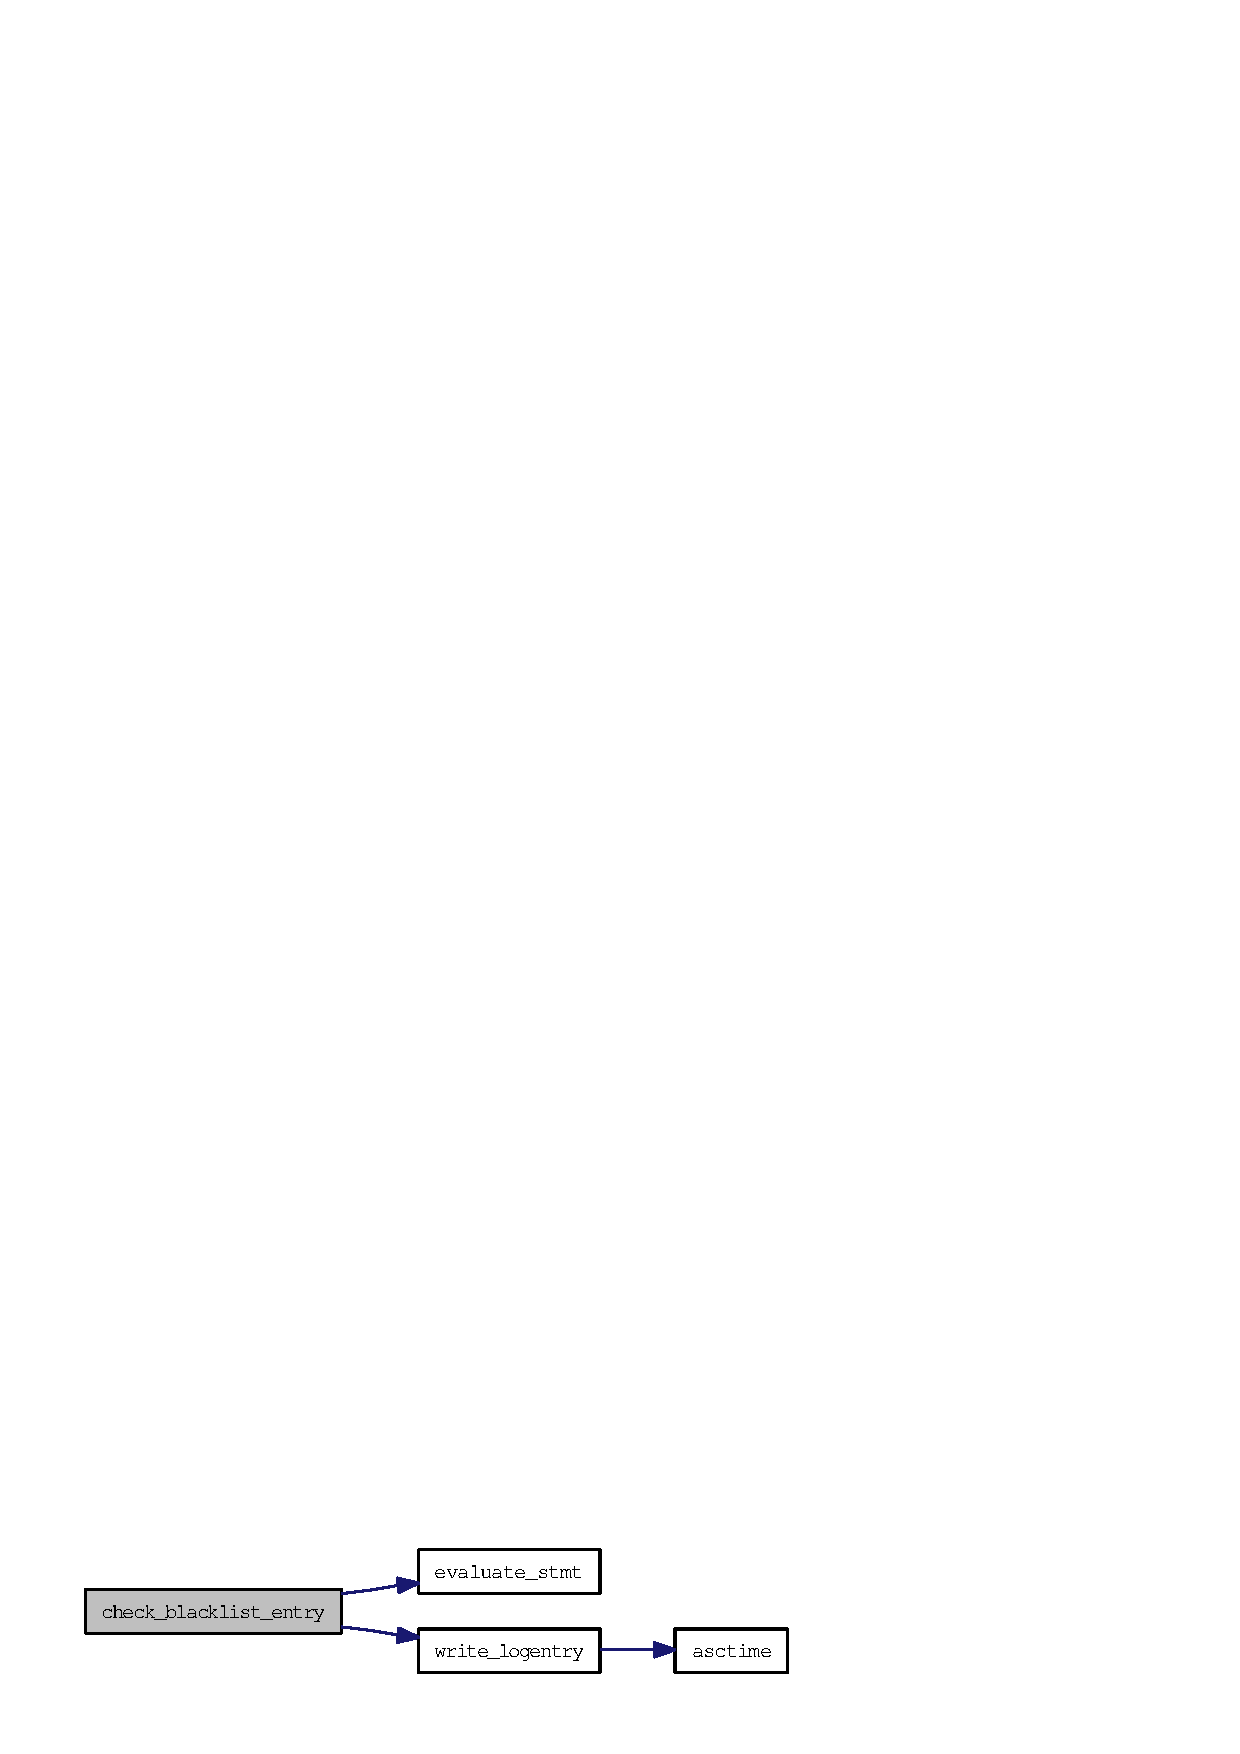
\includegraphics[width=146pt]{libphonefirewall_8h_f28c4b8fd3fdfe5e70df391cf40ca9f2_cgraph}
\end{center}
\end{figure}
\hypertarget{libphonefirewall_8h_f144fe0aa2eb227fe646da21048388a5}{
\index{libphonefirewall.h@{libphonefirewall.h}!check\_\-whitelist\_\-entry@{check\_\-whitelist\_\-entry}}
\index{check\_\-whitelist\_\-entry@{check\_\-whitelist\_\-entry}!libphonefirewall.h@{libphonefirewall.h}}
\subsubsection{\setlength{\rightskip}{0pt plus 5cm}int check\_\-whitelist\_\-entry (int {\em country\_\-code}, int {\em area\_\-code}, unsigned long long {\em number}, int {\em priority})}}
\label{libphonefirewall_8h_f144fe0aa2eb227fe646da21048388a5}


Checks if a number is on the whitelist.

\begin{Desc}
\item[Parameters:]
\begin{description}
\item[{\em country\_\-code}]The country code (for example 39 for Italy, 43 for Austria, and so one) \item[{\em area\_\-code}]The area code which indicates your mobile operator. \item[{\em number}]The telephone number of the person (without country and area code. \item[{\em priority}]Gives the \hyperlink{structentry}{entry} a priority. 0 is standard. If the priority is higher the value will be also blocked/accepted if a higher priority is choosen.\par
 The value \char`\"{}PRIO\_\-ALL\char`\"{} stands for all priorities.\end{description}
\end{Desc}
\begin{Desc}
\item[Returns:]If the number was found 1, otherwise 0. \end{Desc}


Definition at line 261 of file phonefirewall\_\-administration.c.

References Entry::area\_\-code, Entry::country\_\-code, DB\_\-FILE, evaluate\_\-stmt(), Entry::number, Entry::priority, STMT\_\-SIZE, TB\_\-AREACODE, TB\_\-COUNTRYCODE, TB\_\-NUMBER, and TB\_\-PRIORITY.

Here is the call graph for this function:\nopagebreak
\begin{figure}[H]
\begin{center}
\leavevmode
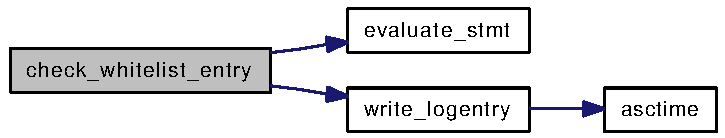
\includegraphics[width=147pt]{libphonefirewall_8h_f144fe0aa2eb227fe646da21048388a5_cgraph}
\end{center}
\end{figure}
\hypertarget{libphonefirewall_8h_04b29323de592cc442250d7c952213de}{
\index{libphonefirewall.h@{libphonefirewall.h}!get\_\-blacklist\_\-entry\_\-by\_\-name@{get\_\-blacklist\_\-entry\_\-by\_\-name}}
\index{get\_\-blacklist\_\-entry\_\-by\_\-name@{get\_\-blacklist\_\-entry\_\-by\_\-name}!libphonefirewall.h@{libphonefirewall.h}}
\subsubsection{\setlength{\rightskip}{0pt plus 5cm}struct {\bf entry}$\ast$ get\_\-blacklist\_\-entry\_\-by\_\-name (char $\ast$ {\em name})\hspace{0.3cm}{\tt  \mbox{[}read\mbox{]}}}}
\label{libphonefirewall_8h_04b29323de592cc442250d7c952213de}


Search a entrie by name.

\begin{Desc}
\item[Parameters:]
\begin{description}
\item[{\em name}]The name of the person which is blocked.\end{description}
\end{Desc}
\begin{Desc}
\item[Returns:]\hyperlink{structentry}{entry} Returns the found \hyperlink{structentry}{entry}. \end{Desc}


Definition at line 27 of file phonefirewall\_\-search.c.\hypertarget{libphonefirewall_8h_80b7f603605d9ea57e83847bed7840f3}{
\index{libphonefirewall.h@{libphonefirewall.h}!get\_\-blacklist\_\-entry\_\-by\_\-number@{get\_\-blacklist\_\-entry\_\-by\_\-number}}
\index{get\_\-blacklist\_\-entry\_\-by\_\-number@{get\_\-blacklist\_\-entry\_\-by\_\-number}!libphonefirewall.h@{libphonefirewall.h}}
\subsubsection{\setlength{\rightskip}{0pt plus 5cm}struct {\bf entry}$\ast$ get\_\-blacklist\_\-entry\_\-by\_\-number (int {\em country\_\-code}, int {\em area\_\-code}, unsigned long long {\em number})\hspace{0.3cm}{\tt  \mbox{[}read\mbox{]}}}}
\label{libphonefirewall_8h_80b7f603605d9ea57e83847bed7840f3}


Search a entrie by number (country code + area code + number).

\begin{Desc}
\item[Parameters:]
\begin{description}
\item[{\em country\_\-code}]The country code (for example 39 for Italy, 43 for Austria, and so one) \item[{\em area\_\-code}]The area code which indicates your mobile operator. \item[{\em number}]The telephone number of the person (without country and area code.\end{description}
\end{Desc}
\begin{Desc}
\item[Returns:]\hyperlink{structentry}{entry} Returns the found \hyperlink{structentry}{entry}. \end{Desc}


Definition at line 30 of file phonefirewall\_\-search.c.\hypertarget{libphonefirewall_8h_f7f20dcd932db52fce6beac057995533}{
\index{libphonefirewall.h@{libphonefirewall.h}!get\_\-whitelist\_\-entry\_\-by\_\-name@{get\_\-whitelist\_\-entry\_\-by\_\-name}}
\index{get\_\-whitelist\_\-entry\_\-by\_\-name@{get\_\-whitelist\_\-entry\_\-by\_\-name}!libphonefirewall.h@{libphonefirewall.h}}
\subsubsection{\setlength{\rightskip}{0pt plus 5cm}struct {\bf entry}$\ast$ get\_\-whitelist\_\-entry\_\-by\_\-name (char $\ast$ {\em name})\hspace{0.3cm}{\tt  \mbox{[}read\mbox{]}}}}
\label{libphonefirewall_8h_f7f20dcd932db52fce6beac057995533}


Search a entrie by name.

\begin{Desc}
\item[Parameters:]
\begin{description}
\item[{\em name}]The name of the person which is accepted.\end{description}
\end{Desc}
\begin{Desc}
\item[Returns:]\hyperlink{structentry}{entry} Returns the found \hyperlink{structentry}{entry}. \end{Desc}


Definition at line 33 of file phonefirewall\_\-search.c.\hypertarget{libphonefirewall_8h_9569cf612525d13ec3443a5df88afe78}{
\index{libphonefirewall.h@{libphonefirewall.h}!get\_\-whitelist\_\-entry\_\-by\_\-number@{get\_\-whitelist\_\-entry\_\-by\_\-number}}
\index{get\_\-whitelist\_\-entry\_\-by\_\-number@{get\_\-whitelist\_\-entry\_\-by\_\-number}!libphonefirewall.h@{libphonefirewall.h}}
\subsubsection{\setlength{\rightskip}{0pt plus 5cm}struct {\bf entry}$\ast$ get\_\-whitelist\_\-entry\_\-by\_\-number (int {\em country\_\-code}, int {\em area\_\-code}, unsigned long long {\em number})\hspace{0.3cm}{\tt  \mbox{[}read\mbox{]}}}}
\label{libphonefirewall_8h_9569cf612525d13ec3443a5df88afe78}


Search a entrie by number (country code + area code + number).

\begin{Desc}
\item[Parameters:]
\begin{description}
\item[{\em country\_\-code}]The country code (for example 39 for Italy, 43 for Austria, and so one) \item[{\em area\_\-code}]The area code which indicates your mobile operator. \item[{\em number}]The telephone number of the person (without country and area code.\end{description}
\end{Desc}
\begin{Desc}
\item[Returns:]\hyperlink{structentry}{entry} Returns the found \hyperlink{structentry}{entry}. \end{Desc}


Definition at line 36 of file phonefirewall\_\-search.c.\hypertarget{libphonefirewall_8h_4eee00c845ad4a60eaccef8c41151ea4}{
\index{libphonefirewall.h@{libphonefirewall.h}!rm\_\-blacklist\_\-entry@{rm\_\-blacklist\_\-entry}}
\index{rm\_\-blacklist\_\-entry@{rm\_\-blacklist\_\-entry}!libphonefirewall.h@{libphonefirewall.h}}
\subsubsection{\setlength{\rightskip}{0pt plus 5cm}int rm\_\-blacklist\_\-entry (int {\em country\_\-code}, int {\em area\_\-code}, unsigned long long {\em number})}}
\label{libphonefirewall_8h_4eee00c845ad4a60eaccef8c41151ea4}


Removes a blocked number from the blacklist.

\begin{Desc}
\item[Parameters:]
\begin{description}
\item[{\em number}]The number which will be deleted.\end{description}
\end{Desc}
\begin{Desc}
\item[Returns:]If all goes right 0, otherwise an error code. \end{Desc}


Definition at line 143 of file phonefirewall\_\-administration.c.

References DB\_\-FILE, STMT\_\-SIZE, TB\_\-AREACODE, TB\_\-COUNTRYCODE, and TB\_\-NUMBER.\hypertarget{libphonefirewall_8h_307d220ee8e63926af279460532787ff}{
\index{libphonefirewall.h@{libphonefirewall.h}!rm\_\-whitelist\_\-entry@{rm\_\-whitelist\_\-entry}}
\index{rm\_\-whitelist\_\-entry@{rm\_\-whitelist\_\-entry}!libphonefirewall.h@{libphonefirewall.h}}
\subsubsection{\setlength{\rightskip}{0pt plus 5cm}int rm\_\-whitelist\_\-entry (int {\em country\_\-code}, int {\em area\_\-code}, unsigned long long {\em number})}}
\label{libphonefirewall_8h_307d220ee8e63926af279460532787ff}


Removes a accepted number from the whitelist.

\begin{Desc}
\item[Parameters:]
\begin{description}
\item[{\em number}]The number which will be deleted.\end{description}
\end{Desc}
\begin{Desc}
\item[Returns:]If all goes right 0, otherwise an error code. \end{Desc}


Definition at line 176 of file phonefirewall\_\-administration.c.

References DB\_\-FILE, STMT\_\-SIZE, TB\_\-AREACODE, TB\_\-COUNTRYCODE, and TB\_\-NUMBER.

\subsection{Variable Documentation}
\hypertarget{libphonefirewall_8h_794ea73ef2f5143bbbb66ebd4c113340}{
\index{libphonefirewall.h@{libphonefirewall.h}!entry@{entry}}
\index{entry@{entry}!libphonefirewall.h@{libphonefirewall.h}}
\subsubsection{\setlength{\rightskip}{0pt plus 5cm}struct {\bf Entry}  {\bf entry}}}
\label{libphonefirewall_8h_794ea73ef2f5143bbbb66ebd4c113340}


